\documentclass[xcolor={dvipsnames,rgb}, aspectratio=169]{beamer}

%%% PACKAGES %%%
\usepackage[T1]{fontenc}
\usepackage{tgheros}

% Metropolis customization
\usetheme[sectionpage=none]{metropolis}
\setbeamercolor{background canvas}{bg=white}
\setbeamercolor{frametitle}{bg = white, fg=black}
\setbeamertemplate{sections/subsections in toc}[square]
\setbeamertemplate{footline}{
   \textcolor{bluepoli}{\rule{\paperwidth}{1pt}}
   \vskip4pt
   \hskip5pt \tiny Numerical Integration $|$ Calcoli di Processo dell' Ingegneria Chimica
   \hskip260pt \insertframenumber
   \vskip4pt
}

% color
\usepackage{color}
\usepackage{xcolor}
\usepackage{colortbl}
\definecolor{bluepoli}{cmyk}{0.4,0.1,0,0.4}
\definecolor{mygreen}{RGB}{1, 121,111}
\definecolor{myred}{RGB}{220, 20, 60}
\definecolor{mygreen}{RGB}{28,172,0}
\definecolor{mylilas}{RGB}{170,55,241}
\definecolor{codegreen}{rgb}{0,0.6,0}
\definecolor{codegray}{rgb}{0.5,0.5,0.5}
\definecolor{codepurple}{rgb}{0.58,0,0.82}
\definecolor{backcolour}{rgb}{0.95,0.95,0.92}
\definecolor{lightblue}{rgb}{56, 167, 232}

\colorlet{colorp}{NavyBlue}
\colorlet{colorT}{WildStrawberry}
\colorlet{colork}{OliveGreen}
\colorlet{colorM}{RoyalPurple}
\colorlet{colorNb}{Plum}
\colorlet{colorIs}{black}
\newcommand{\highlight}[2]{\colorbox{#1!17}{$#2$}}
\newcommand{\highlightdark}[2]{\colorbox{#1!47}{$#2$}}

% tikz
\usepackage{tikz}
\usetikzlibrary{positioning}
\usetikzlibrary{backgrounds}
\usetikzlibrary{arrows,shapes}
\usetikzlibrary{tikzmark}
\usetikzlibrary{calc}

% tcolorbox env
% Coloured box for styling theorems, proof, definitions
\usepackage[most]{tcolorbox}

\newtcolorbox{code}[2][]{
    enhanced jigsaw,
    colframe=bluepoli,
    interior hidden, 
    breakable,
    before skip=10pt,
    after skip=10pt
}

% URL and Hyperref
\usepackage{hyperref}
\hypersetup{
    colorlinks=true,
    linkcolor=blue,
    filecolor=magenta,
    urlcolor=blue,
    pdftitle={Overleaf Example},
    pdfpagemode=FullScreen,
}
\usepackage{url}

% Math stuff
\usepackage{amsmath}
\usepackage{amssymb}
\usepackage{mathtools}
\usepackage{blkarray}
\usepackage{multirow}

% Wrapfig
\usepackage{wrapfig}

% Bibliography
\usepackage[
backend=biber,
style=alphabetic,
sorting=ynt
]{biblatex}
\addbibresource{bibliography.bib}

%%% TITLE %%%
\title{Numerical Integration}
\subtitle{Calcoli di Processo dell' Ingegneria Chimica}
\author[Dinelli, Mehl]{\textbf{Timoteo~Dinelli}, \textbf{Marco~Mehl}}
\institute{
   \inst{} Department of Chemistry, Materials and Chemical Enginering, G. Natta.
   Politecnico di Milano.\\
   email: timoteo.dinelli@polimi.it \\
   email: marco.mehl@polimi.it \\
}
\date{11\textsuperscript{th} of November 2024.}

\newcommand{\norm}[1]{\left\lVert#1\right\rVert}

\begin{document}
% external files inclusion
% Double underline
\def\doubleunderline#1{\underline{\underline{#1}}}

% \newcommand{\zm}{%
%    \begin{bmatrix}
%       X_{11} & X_{12} & \cdots & X_{1p} \\
%       X_{12} & X_{22} & \cdots & X_{2p} \\
%       \vdots & \vdots & \tikzmarknode{Is}{\highlight{colorT}{X_{ij}}} & \vdots \\
%       X_{n1} & X_{n2} & \cdots & X_{np} \\
%    \end{bmatrix}%
% }

\makeatletter
\newcommand{\DrawLine}{%
  \begin{tikzpicture}
  \path[use as bounding box] (0,0) -- (\linewidth,0);
  \draw[color=bluepoli,dashed,dash phase=2pt]
        (0-\kvtcb@leftlower-\kvtcb@boxsep,0)--
        (\linewidth+\kvtcb@rightlower+\kvtcb@boxsep,0);
  \end{tikzpicture}%
  }
\makeatother

{%
   \setbeamertemplate{footline}{}
   \begin{frame}{}
      \maketitle
      \begin{tikzpicture}[overlay, remember picture]
         \node[above left=6.5cm and .01cm of current page.south east] {
         \includegraphics[trim=1cm 1cm 1.5cm 1cm, clip=true, width=6cm]{
            ./../../Introduction to Matlab/slides/figures/_static/ING_IND_INF-eps-converted-to.pdf
         }
      };
      \end{tikzpicture}
   \end{frame}
}

\begin{frame}{Numerical Integration}
   We will discuss several methods to compute (numerically) the integral of a given
   function!
   \begin{itemize}
      \item[$\blacktriangleright$] \textbf{Classical Analysis}:
         \begin{equation*}
            I = \int_{a}^{b} f(x) dx \quad = \quad F(a) - F(b).
         \end{equation*}
         If and only if $F(x)$ is the antiderivative of $f(x)$
         \item[$\blacktriangleright$] \textbf{Numerical Analysis}: Let's build an
            approximation of $f(x)=\Tilde{f}(x)$ by means of a \alert{suitable polynomial}.
            \begin{equation*}
               I = \int_{a}^{b} f(x) dx  \quad \approx \int_{a}^{b} \Tilde{f}(x)dx.
            \end{equation*}
   \end{itemize}
\end{frame}

\begin{frame}{$\Tilde{f}(x)$ as a \alert{Linear} approximation}
   \begin{equation*}
      \Tilde{f}(x) = P(x) = \frac{(b-x)f(a) + (x-a)f(b)}{b-a}
   \end{equation*}
   \begin{equation*}
      I = \int_{a}^{b} f(x) dx \approx \int_{a}^{b} P(x) dx = \frac{1}{2} (b-a)\left[f(a)
      + f(b)\right]
   \end{equation*}

   Trapezoidal interpolation method or Bézout interpolation formula. Generalizing the
   formula can be written as follow:

   \begin{equation*}
      I \approx h \left[0.5f(x_{0}) + f(x_{1}) + f(x_{2}) + ... + f(x_{n-1}) +
      0.5f(x_{n}) \right]
   \end{equation*}
   \begin{equation*}
      h = \frac{b-a}{n} \quad x_{i} = a + i \times h \quad i = 0, 1, ..., n \quad n \geq
      1
   \end{equation*}
\end{frame}

\begin{frame}{$\Tilde{f}(x)$ as a \alert{Quadratic} approximation}

   \begin{equation*}
      \Tilde{f}(x) = P(x) = \frac{(x-c)(x-b)}{2h^{2}}f(a) +
      \frac{(x-a)(x-b)}{-h^{2}}f(c) + \frac{(x-a)(x-c)}{2h^{2}}f(b)
   \end{equation*}
   \begin{equation*}
      I = \int_{a}^{b} f(x) dx \approx \int_{a}^{b} P(x) dx = \frac{h}{3}\left[f(a) + 4f(c)+f(b)\right]
   \end{equation*}
   With:
   \begin{equation*}
      h = \frac{b-a}{2}
   \end{equation*}
   \begin{equation*}
      c = \frac{a+b}{2}
   \end{equation*}
   This is the formula of Simpson or Simpson-Cavalieri.
\end{frame}

\begin{frame}{}
   Generalizing:
   \begin{equation*}
      I \approx
      \frac{h}{3}\left[f(x_{0})+4f(x_{1})+2f(x_{2})+...+2f(x_{n-2})+4f(x_{n-1}+f(x_{n}))\right]
   \end{equation*}

   \begin{equation*}
      h = \frac{b-a}{n} \quad x_{i} = a + i \times h \quad i = 0, 1, ..., n \quad n \in
      \mathbb{N}
   \end{equation*}
\end{frame}

\begin{frame}{Aitken formula}
   It should be noted that, when employing both methods, increasing the number of
   intervals over which the integral is calculated in order to enhance the precision of
   the evaluation does not preclude the utilisation of the preceding iteration's
   evaluations of the function in question (this necessitates the storage of the
   function's value in an array). The ratio between the errors of two successive
   iterations is constant (provided the function is differentiable), indicating a linear
   convergence. Consequently, if the estimate of the integral is evaluated for a number
   of sub-intervals equal to $n$, $2n$, or $4n$, the value of the integral can be
   extrapolated using the following formula:

   \begin{equation*}
      I \approx I_{4n} -
      \frac{\left(I_{4n}-I_{2n}\right)^{2}}{\left(I_{4n}-I_{2n}\right)-\left(I_{2n}-I_{n}\right)}
   \end{equation*}
\end{frame}

%%%%%%%%%%%%%%% EXERCISES
{%
   \setbeamertemplate{footline}{}
   \begin{frame}[standout]
	   Exercises
   \end{frame}
}

\begin{frame}{Exercises}
   \begin{itemize}
      \item[$\blacktriangleright$] Write a MATLAB function to
         perform the numerical integration with the bezout formula and aitken formula.
      \item[$\blacktriangleright$] \textbf{Exercise 1}: A collection tank receive
         polluted water from a variable source. The istantaneous flow rate of the inlet
         dpends on the time of the day according to the following relationship:
         \begin{equation*}
            Q(t) = 2 sin^{2}\left(\frac{t}{24}\pi\right) \quad [l/min]
         \end{equation*}
         At the end of the 24 hours period tank is emptied and the water is moved to a
         treatment facility. Determine the appropriate size of the tank (i.e., the volume
         of the tank).
   \end{itemize}
\end{frame}

\begin{frame}{}
   \begin{itemize}
      \item[$\blacktriangleright$] \textbf{Exercise 2}: The DIPPR database reports the
         following expression for the cp of $SO_{2}$ (T in K, Cp in $[J/kmol K]$). For
         SULFUR DIOXIDE The Ideal Gas Heat Capacity can be calculated as follows:
         \begin{equation*}
            Cp = A + B \times \left(\frac{C}{T \times
            sinh\left(\frac{C}{T}\right)}\right)^{2} + D \times \left(\frac{E}{T \times
            cosh\left(\frac{E}{T}\right)}\right)^{2}
         \end{equation*}
         $A = 3.3375e^{04}$, $B = 2.5864e^{04}$, $C = 9.3280e^{02}$, $D = 1.0880e^{04}$,
         $E = 4.2370e^{02}$ In the range: 100.00 K to 1500.00 K. Using the trapezoidal
         rule, calculate the power necessary to heat 300 $kmol/h$ of $SO_{2}$ from 230 to
         480 $^\circ C$. Calculate the error if we assume the $Cp$ constant at the
         initial temperature, at the average temperature or the final temperature.
   \end{itemize}
\end{frame}

\begin{frame}{}
   \begin{figure}
      \centering
      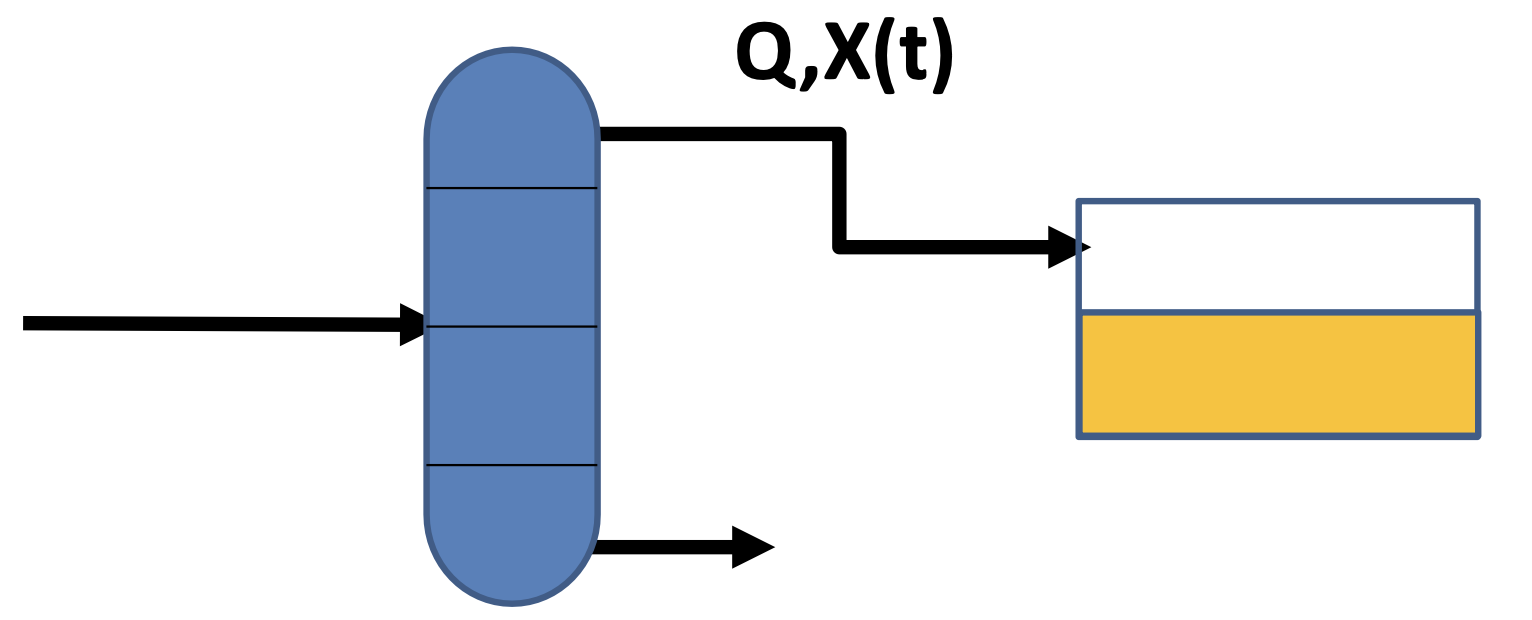
\includegraphics[width=0.5\textwidth]{Schema.png}
   \end{figure}
   \begin{itemize}
      \item[$\blacktriangleright$] \textbf{Exercise 3}: \small{ A distillation process
         enables the recovery of the product, designated as $X$, in a stream that is
         subsequently collected in a tank. The current entering the tank has a constant
         volumetric flow rate, and the concentration of the product $X$ in time is given
         by the following law: $X(t)$ is expressed in $mol/L$, $t$ in hours. }
         \begin{equation*}
            X(t) = sin(\sqrt{t})exp(-2t^{2})
         \end{equation*}
         \small{ The objective is to determine the requisite time for maximizing the
         recovery of component $X$, which has a concentration of 0.3 $mol/L$. The problem
         should be solved using a variety of approaches, including the trapezoidal rule,
         Simpson's rule, and the trapezoidal rule with Aitken extrapolation.}
   \end{itemize}
\end{frame}

\begin{frame}{}
   Total volume recovered in the collection tank
   \begin{equation*}
      V_{tot}(t) = Q t 
   \end{equation*}
   Total moles of $X$ recovered in the collection tank
   \begin{equation*}
      mol_{X_{tot}}(t) = Q \int_{0}^{t}f(x)dx
   \end{equation*}
   Equation solving the problem: a function containing an integral that need to be zeroed
   \begin{equation*}
      C_{X}(t) = \frac{\int_{0}^{t}f(x)dx}{t} = 0.3
   \end{equation*}
\end{frame}

\begin{frame}{}
   \begin{figure}
      \centering
      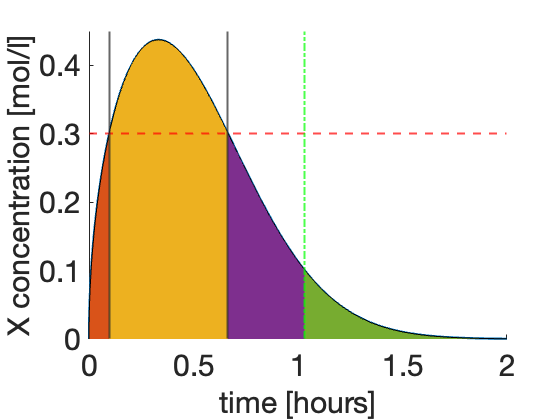
\includegraphics[width=.7\textwidth]{Solution.png}
   \end{figure}
\end{frame}


%%%%%%%%%%%%%%% CLOSING
{%
\setbeamertemplate{footline}{}
\begin{frame}[standout]
	Thank you for the attention!
\end{frame}
}

\end{document}
